\documentclass[
    a4paper,
    12pt,
    addpoints,
    % answers,
    noanswers,
    hidelinks,
]
{exam}

%%% Packages and macros

\usepackage{1-preamble}

%%% Page layout

\input{2-layout}

%%% Subject, paper and conditions

\newcommand{\subject}{Stage 2 Specialist Mathematics}
\newcommand{\papername}{SAT: Stage 1 Review}
\newcommand{\papernameshort}{Stage 1 Review}
\newcommand{\timelimit}{$\infty$~Minutes}
\newcommand{\conditions}{Notes, Calculator}
\newcommand{\paperrules}{\timelimit, \conditions}

\begin{document}

% \input{3-cover-letter}

\begin{questions}

\ifprintanswers
\else
\fullwidth{You and your supervisor must \textbf{write your names} to agree that exam conditions were satisfied.}
\fi

%%% To add: proof of Thales' theorem; proof of law of sines using angle at the centre theorem.

%%% Many of these trig problems have been taken from the old Haese Specialist Maths book.

\question[3]
Let $\sin(\theta) = -\frac{3}{8}$, where $\pi < \theta < \frac{3\pi}{2}$. Find the \emph{exact} value of $\cos(\theta)$ and $\tan(\theta)$.

\begin{EnvFullwidth}
\begin{solutionorgrid}[2in]
The angle $\pi < \theta < \frac{3\pi}{2}$ is in the third quadrant, so $\cos(\theta) < 0$ and $\tan(\theta) > 0$. The right triangle is
\begin{center}
	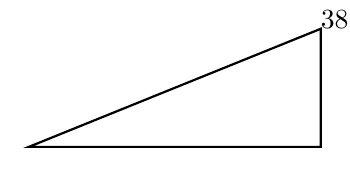
\begin{tikzpicture}[
		scale=.5,
	]
	\coordinate (O) at (0,0);
	\coordinate (A) at (0,-3);
	\coordinate (B) at (-7.416,-3);
	\draw[
	    thick,
	] (O) -- (A) -- (B) -- cycle;
	\tkzLabelSegment[right=.25em](O,A){$3$}
	\tkzLabelSegment[above left=.25em](O,B){$8$}
	\tkzLabelSegment[below=.25em](A,B){$\sqrt{55}$}
	\tkzMarkRightAngle[thick,size=.4](O,A,B)
	\tkzLabelAngle[pos=2](A,B,O){$\theta$}
	\end{tikzpicture}
\end{center}
Thus, $\cos(\theta) = -\frac{\sqrt{55}}{8}$ and $\tan(\theta) = \frac{3}{\sqrt{55}}$.
\end{solutionorgrid}
\end{EnvFullwidth}


\threeast

\question[3]
Without using a calculator, evaluate $\tan^2(\frac{\pi}{6}) + \tan^2(\frac{\pi}{3})$.

\begin{EnvFullwidth}
\begin{solutionorgrid}[2.5in]
We have
\begin{align*}
	\tan^2(\tfrac{\pi}{6}) + \tan^2(\tfrac{\pi}{3}) &= \pfrac{\sin(\frac{\pi}{6})}{\cos(\frac{\pi}{6})}^{\! 2} + \pfrac{\sin(\frac{\pi}{3})}{\cos(\frac{\pi}{3})}^{\! 2} \\
	&= \pfrac{\frac{1}{2}}{\frac{\sqrt{3}}{2}}^{\! 2} + \pfrac{\frac{\sqrt{3}}{2}}{\frac{1}{2}}^{\! 2} \\
	&= \frac{1}{3} + 3 \\
	&= \frac{10}{3}.
\end{align*}
\end{solutionorgrid}
\end{EnvFullwidth}


\triast

\uplevel{
\begin{definition}[General cosine function]
\label{def:general-cosine-function}
Let $A$, $B$, $C$, $D$ and $t$ be real numbers. Then the general cosine function is
\[
	f(t) = A\cos(B(t - C)) + D.
\]
\end{definition}
}

\question
Consider the graph in Figure~\ref{fig:particular-cosine-function} and Definition~\ref{def:general-cosine-function}.

\begin{figure}[h]
	\centering
	\begin{tikzpicture}
	\begin{axis}[
		my axis style,
		ymin=-6,
		ymax=6,
		xlabel={$T$},
		legend pos=north east,
		legend entries={
			$y = f(t)$,
		},
	]
	\addplot[
		domain=-1.5:8.5,
		<->,
	]
	{-4*cos(.5*(pi*x))};
	\draw[
	    thick,
		densely dashed,
		gray,
	]
	(0,4) -| (2,0);
	\end{axis}
	\end{tikzpicture}
	\caption{A particular cosine function.}
	\label{fig:particular-cosine-function}
\end{figure}

\begin{parts}

\part[1]
Find the amplitude $A$ of the graph.

\begin{EnvFullwidth}
\begin{solutionorgrid}[.75in]
The range is from $-4$ to $4$, so the amplitude is $\displaystyle{A = \frac{4 - (-4)}{2} = 4}$.
\end{solutionorgrid}
\end{EnvFullwidth}

\part[1]
State the principal axis $D$ of the graph.

\begin{EnvFullwidth}
\begin{solutionorgrid}[.75in]
We have $\displaystyle{D = \frac{4 + (-4)}{2} = 0}$.
\end{solutionorgrid}
\end{EnvFullwidth}

\part[1]
Find $B$ by considering the period of the graph.

\begin{EnvFullwidth}
\begin{solutionorgrid}[.75in]
The period is $\displaystyle{\frac{2\pi}{B} = 4}$, so $\displaystyle{B = \frac{\pi}{2}}$.
\end{solutionorgrid}
\end{EnvFullwidth}

\part[3]
Find the value of $C$ and hence, find the cosine function whose graph is shown.

\begin{EnvFullwidth}
\begin{solutionorgrid}[1.5in]
We have $f(0) = -4$, so
\begin{align*}
	4\cos(\tfrac{\pi}{2}(0 - C)) + 0 &= -4 \\
	\cos(-\tfrac{C\pi}{2}) &= -1 \\
	\cos(\tfrac{C\pi}{2}) &= -1 \\
	\frac{C\pi}{2} &= \arccos(-1) \\
	\frac{C\pi}{2} &= \pi \\
	C &= 2.
\end{align*}
Thus,
\begin{align*}
	f(t) &= 4\cos(\tfrac{\pi}{2}(t - 2)) \\
	&= 4\cos(\tfrac{\pi}{2} t - \pi) \\
	&= -4\cos(\tfrac{\pi}{2} t).
\end{align*}
\end{solutionorgrid}
\end{EnvFullwidth}

\end{parts}


\threeast

\question
Simplify:

\begin{parts}

\part[1]
$\sin(\theta) - \cos(\frac{\pi}{2} + \theta)$.

\begin{EnvFullwidth}
\begin{solutionorgrid}[1in]
We have
\begin{align*}
	\sin(\theta) - \cos(\tfrac{\pi}{2} + \theta) &= \sin(\theta) - (-\sin(\theta)) \\
	&= 2\sin(\theta).
\end{align*}
\end{solutionorgrid}
\end{EnvFullwidth}

\part[1]
$3\cos(-\theta) - 4\sin(\frac{\pi}{2} - \theta)$.

\begin{EnvFullwidth}
\begin{solutionorgrid}[1.5in]
We have
\begin{align*}
	3\cos(-\theta) - 4\sin(\tfrac{\pi}{2} - \theta) &= 3\cos(\theta) - 4\cos(\theta) \\
	&= -\cos(\theta).
\end{align*}
\end{solutionorgrid}
\end{EnvFullwidth}

\end{parts}


\threeast

\question[3]
Two roads meet at right angles and are $a$~\si{\meter} and $b$~\si{\meter} wide, respectively, as shown in Figure~\ref{fig:two-roads}. Sign posts are positioned at $A$ and $C$. It's known that $A$, $B$ and $C$ are colinear. Show that $AC$ has length $a\sec(\theta) + b\csc(\theta)$.

\begin{figure}[h]
	\centering
	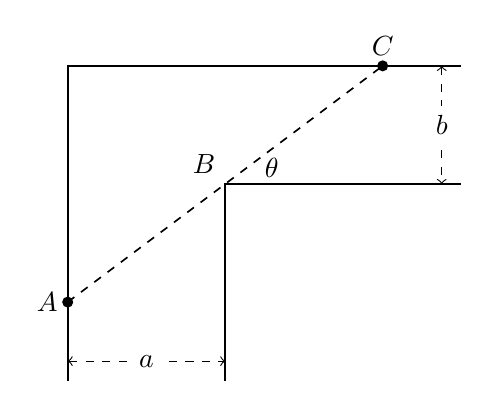
\begin{tikzpicture}
	\coordinate (RTL) at (0,0);
	\coordinate (RTR) at (5,0);
	\coordinate (RBL) at (0,-4);
	\coordinate (RBR) at (2,-4);
	\coordinate (RMR) at (5,-1.5);
	\coordinate (A) at (0,-3);
	\coordinate (B) at (2,-1.5);
	\coordinate (C) at (4,0);
	\draw[
		semithick,
	]
	(RBL) -- (RTL) -- (RTR);
	
	\draw[
		semithick,
	]
	(RBR) -- (B) node[anchor=south east] {$B$} -- (RMR);
	\draw[
		semithick,
		dashed,
	]
	(A) node[anchor=east] {$A$} -- (C) node[anchor=south] {$C$};
	\draw (B) node[above right, xshift=2.5ex, yshift=-.25ex] {$\theta$};
	\draw[
		dashed,
		<->,
	]
	(0,-3.75) -- node[midway,fill=white] {$a$~\si{\meter}} (2,-3.75);
	\draw[
		dashed,
		<->,
	]
	(4.75,0) -- node[midway,fill=white] {$b$~\si{\meter}} (4.75,-1.5);
	\fill[
		black,
	]
	(A) circle (2pt)
	(C) circle (2pt)
	;		
	\end{tikzpicture}
	\caption{The intersection of two roads.}
	\label{fig:two-roads}
\end{figure}

\begin{EnvFullwidth}
\begin{solutionorgrid}[4in]
\begin{center}
	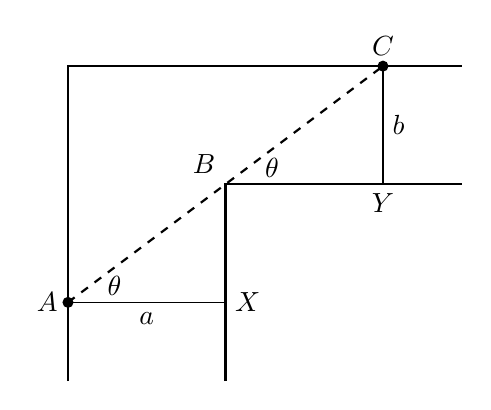
\begin{tikzpicture}
	\coordinate (RTL) at (0,0);
	\coordinate (RTR) at (5,0);
	\coordinate (RBL) at (0,-4);
	\coordinate (RBR) at (2,-4);
	\coordinate (RMR) at (5,-1.5);
	\coordinate (A) at (0,-3);
	\coordinate (B) at (2,-1.5);
	\coordinate (C) at (4,0);
	\coordinate (X) at (2,-3);
	\coordinate (Y) at (4,-1.5);
	\draw[
		thick,
	]
	(RBL) -- (RTL) -- (RTR);
	\draw[
		thick,
	]
	(RBR) -- (B) node[anchor=south east] {$B$} -- (RMR);
	\draw[
		thick,
		dashed,
	]
	(A) node[anchor=east] {$A$} -- (C) node[anchor=south] {$C$};
	\draw (B) node[above right, xshift=2.5ex, yshift=-.25ex] {$\theta$};
	\draw (A) node[above right, xshift=2.5ex, yshift=-.25ex] {$\theta$};
	\draw[
		-,
	]
	(A) -- node[midway, below] {$a$~\si{\meter}} (X);
	\draw[
		-,
	]
	(C) -- node[midway, right] {$b$~\si{\meter}} (Y);
	\fill[
		black,
	]
	(A) circle (2pt)
		(C) circle (2pt)
	;
	\draw (X) node[right] {$X$};
	\draw (Y) node[below] {$Y$};
	\end{tikzpicture}
\end{center}
If $\angle CBY = \theta$, then $\angle BAX = \theta$ and
\[
	\cos(\theta) = \frac{a}{AB},\qquad \sin(\theta) = \frac{b}{BC}.
\]
So,
\begin{align*}
	AB &= \frac{a}{\cos(\theta)} & BC &= \frac{b}{\sin(\theta)} \\
	&= a\sec(\theta), & &= b\csc(\theta).
\end{align*}
Now, $AC = AB + BC$, so $AC = a\sec(\theta) + b\csc(\theta)$, as required.
\end{solutionorgrid}
\end{EnvFullwidth}


\ifprintanswers
\threeast
\else
\newpage
\fi

\question

\begin{parts}

\part
Simplify:

\begin{subparts}

\subpart[2]
$\csc(x) - \cos(x)\cot(x)$. (\emph{Hint}: $\cos^2(x) + \sin^2(x) = 1$.)

\begin{EnvFullwidth}
\begin{solutionorgrid}[1.5in]
We have
\begin{align*}
	\csc(x) - \cos(x)\cot(x) &= \frac{1}{\sin(x)} - \cos(x) \frac{\cos(x)}{\sin(x)} \\
	&= \frac{1 - \cos^2(x)}{\sin(x)} \\
	&= \frac{\sin^2(x)}{\sin(x)} \\
	&= \sin(x).
\end{align*}
\end{solutionorgrid}
\end{EnvFullwidth}

\subpart[3]
$\displaystyle{\frac{\sin(\theta) + \tan(\theta)}{1 + \cos(\theta)}}$. (\emph{Hint}: $\displaystyle{\tan(\theta) = \frac{\sin(\theta)}{\cos(\theta)}}$.)

\begin{EnvFullwidth}
\begin{solutionorgrid}[3in]
We have
\begin{align*}
	\frac{\sin(\theta) + \tan(\theta)}{1 + \cos(\theta)} &= \frac{\sin(\theta) + \frac{\sin(\theta)}{\cos(\theta)}}{1 + \cos(\theta)} \\
	&= \frac{\sin(\theta) \cos(\theta) + \sin(\theta)}{\cos(\theta)(1 + \cos(\theta))} \\
	&= \frac{\sin(\theta) (\cancel{\cos(\theta) + 1)}}{\cos(\theta)(\cancel{1 + \cos(\theta)})} \\
	&= \tan(\theta).
\end{align*}
\end{solutionorgrid}
\end{EnvFullwidth}

\end{subparts}

\part[3] %%% New Haese Ex 4F.3, Q3g).
Show that $\displaystyle{\frac{\cos(\alpha)}{1 - \tan(\alpha)} + \frac{\sin(\alpha)}{1 - \cot(\alpha)} = \cos(\alpha)} + \sin(\alpha)$. (\emph{Hint}: difference of two squares.)

\begin{EnvFullwidth}
\begin{solutionorgrid}[3.25in]
The LHS is
\begin{align*}
    \frac{\cos(\alpha)}{1 - \frac{\sin(\alpha)}{\cos(\alpha)}} + \frac{\sin(\alpha)}{1 - \frac{\cos(\alpha)}{\sin(\alpha)}}
    &=
    \frac{\cos(\alpha)}{\frac{\cos(\alpha) - \sin(\alpha)}{\cos(\alpha)}} + \frac{\sin(\alpha)}{\frac{\sin(\alpha) - \cos(\alpha)}{\sin(\alpha)}} \\
    &=
    \frac{\cos^2(\alpha)}{\cos(\alpha) - \sin(\alpha)} + \frac{\sin^2(\alpha)}{\sin(\alpha) - \cos(\alpha)} \\
    &=
    \frac{\cos^2(\alpha)}{\cos(\alpha) - \sin(\alpha)} - \frac{\sin^2(\alpha)}{\cos(\alpha) - \sin(\alpha)} \\
    &=
    \frac{\cancel{(\cos(\alpha) - \sin(\alpha))}(\cos(\alpha) + \sin(\alpha))}{\cancel{(\cos(\alpha) - \sin(\alpha))}},
\end{align*}
which is the RHS.
\end{solutionorgrid}
\end{EnvFullwidth}

\end{parts}


\ifprintanswers
\threeast
\else
\newpage
\fi

\uplevel{
\begin{theorem}[Difference of sine squares]
\label{thm:difference-of-sine-squares}
Let $\theta$ and $\varphi$ be real numbers. Then
\[
	\sin^2(\theta) - \sin^2(\varphi) = \sin(\theta + \varphi)\sin(\theta - \varphi).
\]
\end{theorem}
}

\question[4]
Prove Theorem~\ref{thm:difference-of-sine-squares}.

\begin{EnvFullwidth}
\begin{solutionorgrid}[5in]
\begin{proof}
Let $A = \sin(\theta + \varphi)$ and $B = \sin(\theta - \varphi)$. By the angle sum identities
\[
	A = \sin(\theta)\cos(\varphi) + \sin(\varphi)\cos(\theta),
\]
and
\[
	B = \sin(\theta)\cos(\varphi) - \sin(\varphi)\cos(\theta).
\]
Thus
\begin{align*}
	AB &= (\sin(\theta)\cos(\varphi) + \sin(\varphi)\cos(\theta)) \times (\sin(\theta)\cos(\varphi) - \sin(\varphi)\cos(\theta)) \\
	&= (\sin(\theta)\cos(\varphi))^2 - \sin(\theta)\sin(\varphi)\cos(\theta)\cos(\varphi) + \sin(\theta)\sin(\varphi)\cos(\theta)\cos(\varphi) - (\sin(\varphi)\cos(\theta))^2 \\
	&= \sin^2(\theta)\cos^2(\varphi) - \sin^2(\varphi)\cos^2(\theta) \\
	&= \sin^2(\theta)(1 - \sin^2(\varphi)) - \sin^2(\varphi)(1 - \sin^2(\theta)) \\
	&= \sin^2(\theta) - \sin^2(\theta)\sin^2(\varphi) - \sin^2(\varphi) + \sin^2(\theta)\sin^2(\varphi) \\
	&= \sin^2(\theta) - \sin^2(\varphi).
\end{align*}
\end{proof}
\end{solutionorgrid}
\end{EnvFullwidth}


\triast

\uplevel{
\begin{theorem}[Sum of geometric sequence]
\label{thm:sum-of-geometric-sequence}
Let $r \neq 1$ be be a real number and let $n$ be a positive integer. Then
\[
    1 + r + r^2 + r^3 + \cdots + r^{n - 1} = \frac{r^n - 1}{r - 1}.
\]
Note that this could equivalently be written, using sigma summation notation, as
\[
    \sum_{j = 0}^{n - 1} r^j = \frac{r^n - 1}{r - 1}.
\]
\end{theorem}
}

\question

\begin{parts}

\part[5] % RS 6A, Q1c).
Prove Theorem~\ref{thm:sum-of-geometric-sequence} by mathematical induction.

\begin{EnvFullwidth}
\begin{solutionorgrid}[4.5in]
\begin{proof}
$P(n)$ is: $\displaystyle{\sum_{j = 0}^{n - 1} r^j = \frac{r^n - 1}{r - 1}}$, for all $n \in \Z^+$.

\textbf{Basis}: If $n = 1$, the LHS is $r^{1 - 1} = r^0 = 1$ and the RHS is $\displaystyle{\frac{r^1 - 1}{r - 1}} = 1$. So $P(1)$ is true.

\textbf{Inductive step}: If $P(k)$ is true then $\displaystyle{\sum_{j = 0}^{k - 1} r^j = \frac{r^k - 1}{r - 1}}$, for all $k \in \Z^+$. Now,
\begin{align*}
    \sum_{j = 0}^k r^j &= \frac{r^k - 1}{r - 1} + r^{k} && (\textrm{by hypothesis}) \\
    &= \frac{r^k - 1}{r - 1} + \frac{r^{k}(r - 1)}{(r - 1)} \\
    &= \frac{r^k - 1 + r^{k + 1} - r^k}{r - 1} \\
    &= \frac{r^{k + 1} - 1}{r - 1}.
\end{align*}
Since $P(1)$ is true and $P(k) \implies P(k + 1)$, by the PMI, $P(n)$ is true for all $n \in \Z^+$.
\end{proof}
\end{solutionorgrid}
\end{EnvFullwidth}

\part[2]
Hence, find $\displaystyle{1 + \frac{1}{2} + \frac{1}{4} + \frac{1}{8} + \cdots + \frac{1}{256} = \sum_{j = 0}^{8} \pfrac{1}{2}^{\! j}.}$ in the form $\displaystyle{\frac{m}{n}}$.

\begin{EnvFullwidth}
\begin{solutionorgrid}[2.5in]
By Theorem~\ref{thm:sum-of-geometric-sequence}, on putting $r = \frac{1}{2}$ and $n - 1 = 8$ we get
\begin{align*}
    \sum_{j = 0}^{8} \pfrac{1}{2}^{\! j} &= \frac{(\frac{1}{2})^9 - 1}{\frac{1}{2} - 1} \\
    &= \frac{\frac{1}{512} - \frac{512}{512}}{-\frac{1}{2}} \\
    &= \frac{-\frac{511}{512}}{-\frac{1}{2}} \\
    &= \frac{511}{256}.
\end{align*}
\end{solutionorgrid}
\end{EnvFullwidth}

\end{parts}


\threeast

\question % Ex. 6F, Q1.
Let $n$ be a positive integer and let
\[
    \mat{A} =
    \begin{pmatrix}
        1 & 2 \\
        0 & 1
    \end{pmatrix}
\]
be a matrix.

\begin{parts}

\part[3]
Find $\mat{A}^n$, for $n = 2$, $n = 3$ and $n = 4$.

\begin{EnvFullwidth}
\begin{solutionorgrid}[2.5in]
For $n = 2$
\[
    \mat{A}^2
    =
    \begin{pmatrix}
        1 & 2 \\
        0 & 1
    \end{pmatrix}
    \begin{pmatrix}
        1 & 2 \\
        0 & 1
    \end{pmatrix}
    =
    \begin{pmatrix}
        1 & 4 \\
        0 & 1
    \end{pmatrix}.
\]
For $n = 3$
\[
    \mat{A}^3 = \mat{A}^2\mat{A}
    =
    \begin{pmatrix}
        1 & 4 \\
        0 & 1
    \end{pmatrix}
    \begin{pmatrix}
        1 & 2 \\
        0 & 1
    \end{pmatrix}
    =
    \begin{pmatrix}
        1 & 6 \\
        0 & 1
    \end{pmatrix}.
\]
For $n = 4$
\[
    \mat{A}^4 = \mat{A}^3\mat{A}
    =
    \begin{pmatrix}
        1 & 6 \\
        0 & 1
    \end{pmatrix}
    \begin{pmatrix}
        1 & 2 \\
        0 & 1
    \end{pmatrix}
    =
    \begin{pmatrix}
        1 & 8 \\
        0 & 1
    \end{pmatrix}.
\]
\end{solutionorgrid}
\end{EnvFullwidth}

\part[1]
Make a conjecture about the value of $\mat{A}^n$, for all positive integers $n$.

\begin{EnvFullwidth}
\begin{solutionorgrid}[.75in]
\textbf{Conjecture}. For all $n \in \Z^+$ we have
\[
    \mat{A}^n =
    \begin{pmatrix}
        1 & 2n \\
        0 & 1
    \end{pmatrix}.
\]
\end{solutionorgrid}
\end{EnvFullwidth}

\part[5] % RS 6A, Q1c).
Prove your conjecture in (b) by mathematical induction.

\begin{EnvFullwidth}
\begin{solutionorgrid}[4.5in]
\begin{proof}
$P(n)$ is:
\[
    \mat{A}^n =
    \begin{pmatrix}
        1 & 2n \\
        0 & 1
    \end{pmatrix}
\]
for all $n \in \Z^+$.

\textbf{Basis}: If $n = 1$, the LHS is clearly equal to the RHS. So $P(1)$ is true.

\textbf{Inductive step}: If $P(k)$ is true then
\[
    \mat{A}^k =
    \begin{pmatrix}
        1 & 2k \\
        0 & 1
    \end{pmatrix}
\]
for all $k \in \Z^+$. Now,
\begin{align*}
    \mat{A}^{k + 1} &= \mat{A}^k\mat{A} \\
    &=
    \begin{pmatrix}
        1 & 2k \\
        0 & 1
    \end{pmatrix}
    \begin{pmatrix}
        1 & 2 \\
        0 & 1
    \end{pmatrix} && (\textrm{by hypothesis}) \\
    &=
    \begin{pmatrix}
        1 & 2 + 2k \\
        0 & 1
    \end{pmatrix} \\
    &=
    \begin{pmatrix}
        1 & 2(k + 1) \\
        0 & 1
    \end{pmatrix}.
\end{align*}
Since $P(1)$ is true and $P(k) \implies P(k + 1)$, by the PMI, $P(n)$ is true for all $n \in Z^+$.
\end{proof}
\end{solutionorgrid}
\end{EnvFullwidth}

\end{parts}


\triast

\uplevel{
\begin{proposition}[Bisector is perpendicular]
\label{prop:bisector-is-perpendicular}
The line joining the apex to the midpoint of the base of an isosceles triangle is perpendicular to the base.
\end{proposition}
}

\question % Ex. 3L, Q7.
Consider isosceles triangle $OAB$ shown in Figure~\ref{fig:bisector-is-perpendicular}. Let $\vv{OA} = \vec{a}$ and $\vv{OB} = \vec{b}$.

\begin{figure}[h]
    \centering
    \begin{tikzpicture}
    \tkzDefPoint(0,0){O}
    \tkzDefShiftPoint[O](240:4.5){A}
    \tkzDefShiftPoint[O](300:4.5){B}
    \tkzDefMidPoint(A,B)
    \tkzGetPoint{M}
    \tkzLabelPoint[right](O){$O$}
    \tkzLabelPoint[left](A){$A$}
    \tkzLabelPoint[right](B){$B$}
    \tkzLabelPoint[below](M){$M$}
    \ifprintanswers
    \tkzDrawSegments[vector,color=red](O,A O,B O,M A,B)
    \tkzMarkSegment[mark=|,color=red](O,A)
    \tkzMarkSegment[mark=|,color=red](O,B)
    \tkzMarkSegment[mark=||,color=red](A,M)
    \tkzMarkSegment[mark=||,color=red](B,M)
    \tkzLabelSegment[pos=.6,left,color=red](O,A){$\vec{a}$}
    \tkzLabelSegment[pos=.6,right,color=red](O,B){$\vec{b}$}
    \tkzLabelSegment[pos=.6,left,color=red](O,M){$\vv{OM}$}
    \else
    \tkzMarkSegment[mark=|](O,A)
    \tkzMarkSegment[mark=|](O,B)
    \tkzMarkSegment[mark=||](A,M)
    \tkzMarkSegment[mark=||](B,M)
    \tkzDrawPolygon[semithick](O,A,B)
    \tkzDrawPoint(M)
    \fi
    \end{tikzpicture}
    \caption{Isosceles triangle $ABC$.}
    \label{fig:bisector-is-perpendicular}
\end{figure}

\begin{parts}

\part[1]
Draw vector $\vv{OM}$ on Figure~\ref{fig:bisector-is-perpendicular}.

\part[2]
Find $\vv{AB}$ and $\vv{OM}$ in terms of $\vec{a}$ and $\vec{b}$.

\begin{EnvFullwidth}
\begin{solutionorgrid}[2in]
We have
\[
    \vv{AB} = \vec{b} - \vec{a},
\]
and
\[
    \vv{OM} = \vv{OA} + \frac{1}{2}\vv{AB} = \vec{a} + \frac{1}{2}(\vec{b} - \vec{a}) = \frac{1}{2}(\vec{b} + \vec{a}).
\]
\end{solutionorgrid}
\end{EnvFullwidth}

\part[3]
Hence, use vectors to prove Proposition~\ref{prop:bisector-is-perpendicular}.

\begin{EnvFullwidth}
\begin{solutionorgrid}[2.5in]
\begin{proof}
We have
\begin{align*}
    \vv{OM} \cdot \vv{AB} &= \frac{1}{2}(\vec{b} + \vec{a}) \cdot (\vec{b} - \vec{a}) && (\textrm{by (b)}) \\
    &= \frac{1}{2}(\vec{b} \cdot \vec{b} \cancel{- \vec{b} \cdot \vec{a} + \vec{a} \cdot \vec{b}} - \vec{a} \cdot \vec{a}) \\
    &= \abs{\vec{b}}^2 - \abs{\vec{a}}^2 \\
    &= 0 && (\triangle OAB \textrm{ is isosceles}).
\end{align*}
A zero dot product implies perpendicularity.
\end{proof}
\end{solutionorgrid}
\end{EnvFullwidth}

\end{parts}


\ifprintanswers
\threeast
\else
\fi

\begin{theorem}[Law of sines]
\label{thm:law-of-sines}
Let triangle $ABC$ have sides of length $a$, $b$ and $c$ and angles $\alpha$, $\beta$ and $\gamma$. Let $R$ be the radius of the circumcircle of triangle $ABC$. Then we have
\[
    \frac{a}{\sin(\alpha)} = \frac{b}{\sin(\beta)} = \frac{c}{\sin(\gamma)} = 2R.
\]
\end{theorem}

\question
Theorem~\ref{thm:law-of-sines} will be proved using Figure~\ref{fig:law-of-sines} as a starting point. (\emph{Note}: we'll use side $a$ and angle $\alpha$ but the argument will apply equally well to the other side and angle pairs.)

\begin{figure}[h]
    \centering
    \begin{tikzpicture}
    \tkzDefPoints{0/0/A, 5/2/B, 1/5/C}
    \tkzDefCircle[circum](A,B,C)
    \tkzGetPoint{O} \tkzGetLength{rO}
    \tkzDefPointOnCircle[angle=-45,center=O,radius=\rO pt]
    \tkzGetPoint{P}
    \tkzDefMidPoint(B,C) \tkzGetPoint{M}
    \tkzDrawPolygon[semithick](A,B,C)
    \tkzDrawCircle[semithick](O,A)
    \ifprintanswers
    \tkzDrawSegment[dim={$a$,24pt,above=6pt}](C,B)
    \tkzDrawSegments[semithick,color=brown](O,B O,C)
    \tkzDrawSegment[semithick,color=blue](O,M)
    \tkzDrawPoints(M)
    \tkzMarkSegments[mark=|,color=brown](O,B O,C)
    \tkzMarkSegments[pos=.75,mark=|,color=brown](O,P)
    \tkzMarkSegments[mark=||,color=blue](B,M C,M)
    \tkzMarkRightAngle[color=gray](B,M,O)
    \tkzMarkAngles[size=20pt,mark=none,color=gray](B,A,C B,O,M)
    \tkzLabelAngle[pos=.5](B,O,M){$\alpha$}
    \tkzLabelPoint[above right](M){$M$}
    \else
    \fi
    \tkzDrawSegment[dim={$a$,24pt,above=6pt}](C,B)
    \tkzDrawSegments[semithick,color=brown](O,P)
    \tkzDrawPoints(A,B,C,O,P)
    \tkzLabelPoint[left](A){$A$}
    \tkzLabelPoint[right](B){$B$}
    \tkzLabelPoint[above](C){$C$}
    \tkzLabelPoint[left](O){$O$}
    \tkzLabelAngle[pos=.5](B,A,C){$\alpha$}
    % \tkzLabelSegment[left](A,C){$b$}
    % \tkzLabelSegment[below](A,B){$c$}
    \tkzLabelSegment[pos=.75,color=brown](O,P){$R$}
    \end{tikzpicture}
    \caption{The circumcircle of triangle $ABC$ passes through its three vertices.}
    \label{fig:law-of-sines}
\end{figure}

\begin{parts}

\part[1]
Form triangle $BOC$ by drawing line segments $BO$ and $CO$ on Figure~\ref{fig:law-of-sines}.

\part[1]
Find the measure of $\angle BOC$.

\begin{EnvFullwidth}
\begin{solutionorgrid}[.75in]
By the angle at the centre theorem, $\angle BOC = 2\alpha$.
\end{solutionorgrid}
\end{EnvFullwidth}

\part[2]
Let $M$ be the midpoint of line segment $BC$. Explain why $\angle OMB = \ang{90}$.

\begin{EnvFullwidth}
\begin{solutionorgrid}[1in]
Since $ABC$ is an isosceles triangle, the altitude has the midpoint as its foot.
\end{solutionorgrid}
\end{EnvFullwidth}

\part[2]
Explain why $\angle MOB = \alpha$.

\begin{EnvFullwidth}
\begin{solutionorgrid}[1.5in]
The altitude of an isosceles triangle bisects the angle at the vertex. Thus,
\[
    \angle MOB = \frac{1}{2} \angle BOC = \alpha.
\]
\end{solutionorgrid}
\end{EnvFullwidth}

\part[2]
Using these results, prove Theorem~\ref{thm:law-of-sines}.

\begin{EnvFullwidth}
\begin{solutionorgrid}[2in]
\begin{proof}
Using the earlier results, in triangle $MOB$ we have
\begin{align*}
    \sin(\alpha) &= \frac{a/2}{R} \\
    R\sin(\alpha) &= \frac{a}{2} \\
    \frac{a}{\sin(\alpha)} &= 2R.
\end{align*}
\end{proof}
\end{solutionorgrid}
\end{EnvFullwidth}

\end{parts}


\triast

\uplevel{
\begin{theorem}[Product of complex conjugates]
\label{thm:product-of-complex-conjugates}
Let $a$ and $b$ be real numbers and let $z = a + bi$ be a complex number. Then $\conj{z} = a - bi$ is the complex conjugate of $z$ and
\[
    z\conj{z} = \abs{z}^2.
\]
\end{theorem}
}

\question % Ex. 7I.2, Q5.

\begin{parts}

\part[3]
Prove Theorem~\ref{thm:product-of-complex-conjugates}.

\begin{EnvFullwidth}
\begin{solutionorgrid}[3in]
\begin{proof}
The LHS is
\begin{align*}
    z\conj{z} &= (a + bi)(a - bi) \\
    &= a^2 - b^2i^2 \\
    &= a^2 + b^2.
\end{align*}
The RHS is
\[
    (\sqrt{a^2 + b^2})^2 = a^2 + b^2.
\]
This completes the proof.
\end{proof}
\end{solutionorgrid}
\end{EnvFullwidth}

\uplevel{
Let $w$ be a complex number such that $\abs{w} = 2\sqrt{10}$ and such that $w$ satisfies the equation
\[
    \frac{50}{\conj{w}} - \frac{10}{w} = 2 + 9i.
\]
}

\ifprintanswers
\else
\newpage
\fi
\part[5]
Find $w$.

\begin{EnvFullwidth}
\begin{solutionorgrid}[4.5in]
The LHS is
\begin{align*}
    \frac{50w - 10\conj{w}}{\conj{w}w} &= \frac{50w - 10\conj{w}}{\abs{w}^2} && (\textrm{By Theorem~\ref{thm:product-of-complex-conjugates}}) \\
    &= \frac{50w - 10\conj{w}}{4 \times 10} && (\abs{w} = 2\sqrt{10}).
\end{align*}
Let $w = c + di$ so $\conj{w} = c - di$. Thus
\begin{align*}
    50w - 10\conj{w} &= 40(2 + 9i) \\
    5(c + di) - (c - di) &= 4(2 + 9i) \\
    4c + 6di &= 8 + 36i.
\end{align*}
By comparing real and imaginary parts
\[
    c = 2, \qquad d = 6.
\]
\end{solutionorgrid}
\end{EnvFullwidth}

\end{parts}


\threeast

\question

\begin{parts}

\part[2] % RS 7B, Q4c).
Find integers $a$ and $b$ such that $\displaystyle{\frac{1}{(\sqrt{2} + 1)^2} = a + b\sqrt{2}}$.

\begin{EnvFullwidth}
\begin{solutionorgrid}[3.5in]
We have
\begin{align*}
    \frac{1}{2 + 2\sqrt{2} + 1} &= \frac{1}{3 + 2\sqrt{2}} \times \frac{3 - 2\sqrt{2}}{3 - 2\sqrt{2}} \\
    &= \frac{3 - 2\sqrt{2}}{9 \cancel{- 6\sqrt{12} + 6\sqrt{12}} - 4 \times 2} \\
    &= \frac{3 - 2\sqrt{2}}{1}.
\end{align*}
Thus, $a = 3$ and $b = -2$.
\end{solutionorgrid}
\end{EnvFullwidth}

\part[4] % RS 7B, Q10.
Find rational numbers $p$ and $q$ such that $\displaystyle{\frac{2 - 3i}{2p + qi} = 3 + 2i}$.

\begin{EnvFullwidth}
\begin{solutionorgrid}[4in]
We have
\begin{align*}
    \frac{2 - 3i}{2p + qi} &= 3 + 2i \\
    2 - 3i &= (3 + 2i)(2p + qi) && (2p + qi \neq 0) \\
    2 - 3i &= 6p + 3qi + 4pi + 2qi^2  \\
    2 - 3i &= 2(3p - q) + i(4p + 3q).
\end{align*}
On comparing real and imaginary parts we get
\begin{gather*}
    \systeme{
        3p - q = 1@\qquad(*),
        4p + 3q = -3
    }
\end{gather*}
then on multiplying (1) by $3$, then adding the equations yields $13p = 0$, so $p = 0$. Thus, $q = -1$.
\end{solutionorgrid}
\end{EnvFullwidth}

\end{parts}


\end{questions}

\vfill

\input{8-grading-table}

\input{9-formulae-sheet}

\end{document}
